\documentclass[]{report}
\usepackage{lmodern}
\usepackage{amssymb,amsmath}
\usepackage{ifxetex,ifluatex}
\usepackage{fixltx2e} % provides \textsubscript
\ifnum 0\ifxetex 1\fi\ifluatex 1\fi=0 % if pdftex
  \usepackage[T1]{fontenc}
  \usepackage[utf8]{inputenc}
\else % if luatex or xelatex
  \ifxetex
    \usepackage{mathspec}
  \else
    \usepackage{fontspec}
  \fi
  \defaultfontfeatures{Ligatures=TeX,Scale=MatchLowercase}
\fi
% use upquote if available, for straight quotes in verbatim environments
\IfFileExists{upquote.sty}{\usepackage{upquote}}{}
% use microtype if available
\IfFileExists{microtype.sty}{%
\usepackage{microtype}
\UseMicrotypeSet[protrusion]{basicmath} % disable protrusion for tt fonts
}{}
\usepackage[margin=1in]{geometry}
\usepackage{hyperref}
\hypersetup{unicode=true,
            pdfauthor={Samuel Lippl},
            pdfborder={0 0 0},
            breaklinks=true}
\urlstyle{same}  % don't use monospace font for urls
\usepackage{natbib}
\bibliographystyle{apalike}
\usepackage{longtable,booktabs}
\usepackage{graphicx,grffile}
\makeatletter
\def\maxwidth{\ifdim\Gin@nat@width>\linewidth\linewidth\else\Gin@nat@width\fi}
\def\maxheight{\ifdim\Gin@nat@height>\textheight\textheight\else\Gin@nat@height\fi}
\makeatother
% Scale images if necessary, so that they will not overflow the page
% margins by default, and it is still possible to overwrite the defaults
% using explicit options in \includegraphics[width, height, ...]{}
\setkeys{Gin}{width=\maxwidth,height=\maxheight,keepaspectratio}
\IfFileExists{parskip.sty}{%
\usepackage{parskip}
}{% else
\setlength{\parindent}{0pt}
\setlength{\parskip}{6pt plus 2pt minus 1pt}
}
\setlength{\emergencystretch}{3em}  % prevent overfull lines
\providecommand{\tightlist}{%
  \setlength{\itemsep}{0pt}\setlength{\parskip}{0pt}}
\setcounter{secnumdepth}{5}

%%% Use protect on footnotes to avoid problems with footnotes in titles
\let\rmarkdownfootnote\footnote%
\def\footnote{\protect\rmarkdownfootnote}

%%% Change title format to be more compact
\usepackage{titling}

% Create subtitle command for use in maketitle
\newcommand{\subtitle}[1]{
  \posttitle{
    \begin{center}\large#1\end{center}
    }
}

\setlength{\droptitle}{-2em}

  \title{}
    \pretitle{\vspace{\droptitle}}
  \posttitle{}
    \author{Samuel Lippl}
    \preauthor{\centering\large\emph}
  \postauthor{\par}
      \predate{\centering\large\emph}
  \postdate{\par}
    \date{2018-08-27}

\usepackage{booktabs, titlesec, blindtext}
\usepackage[svgnames]{xcolor}
\hypersetup{
    bookmarksnumbered=true,
    bookmarksopen=false,
    bookmarksopenlevel=1,
    colorlinks=true,
    linkcolor=blue,
    urlcolor=DarkBlue,
    citecolor=DarkRed
}
\definecolor{chgray}{gray}{0.5}
\newcommand{\hsp}{\hspace{20pt}}
\titleformat{\chapter}[hang]{\Huge\bfseries}{\thechapter\hsp\textcolor{chgray}{|}\hsp}{0pt}{\Huge\bfseries}

\usepackage{amsthm}
\newtheorem{theorem}{Theorem}[chapter]
\newtheorem{lemma}{Lemma}[chapter]
\theoremstyle{definition}
\newtheorem{definition}{Definition}[chapter]
\newtheorem{corollary}{Corollary}[chapter]
\newtheorem{proposition}{Proposition}[chapter]
\theoremstyle{definition}
\newtheorem{example}{Example}[chapter]
\theoremstyle{definition}
\newtheorem{exercise}{Exercise}[chapter]
\theoremstyle{remark}
\newtheorem*{remark}{Remark}
\newtheorem*{solution}{Solution}
\begin{document}

\begin{titlepage}

% Titlepage inspired by: https://www.overleaf.com/15991102jmmvbxxtbhfk#/61015645/

\newcommand{\HRule}{\rule{\linewidth}{0.5mm}} % Defines a new command for the horizontal lines, change thickness here

\center % Center everything on the page

%----------------------------------------------------------------------------------------
%	TITLE SECTION
%----------------------------------------------------------------------------------------

\HRule \\[0.4cm]
{ \huge \bfseries Outler Detection using Regression in R}\\[0.4cm] % Title of your document
\HRule \\[1.5cm]

%----------------------------------------------------------------------------------------
%	HEADING SECTIONS
%----------------------------------------------------------------------------------------

\textsc{\LARGE Ludwig-Maximilians-Universität München}\\[0.5cm] % Name of your university/college
\textsc{\Large Fakultät für Mathematik, Informatik und Statistik}\\[1.5cm]


\textsc{\Large Seminar "`Ausreißer- und Anomaliedetektion"' von Prof. Dr. Christian Heumann}\\[0.5cm] % Major heading such as course name
\textsc{\large Hausarbeit}\\[0.5cm] % Minor heading such as course title

%----------------------------------------------------------------------------------------
%	LOGO SECTION
%----------------------------------------------------------------------------------------

\vfill


\includegraphics[height=0.2\textheight]{figs/sigill.png}\\[1cm] % Include a department/university logo - this will require the graphicx package



%----------------------------------------------------------------------------------------
%	DATE SECTION
%----------------------------------------------------------------------------------------

\vfill

%----------------------------------------------------------------------------------------
%	AUTHOR SECTION
%----------------------------------------------------------------------------------------

{\Large 30. Juni 2018}\\[1cm]
\begin{Large}
\textsc{Autor}\\Samuel Lippl
\end{Large}

\vfill

\end{titlepage}

\pagenumbering{roman}
\setcounter{page}{2}

\chapter*{Selbständigkeitserklärung}

Ich erkläre hiermit, dass ich die vorliegende Arbeit selbständig angefertigt, alle Zitate als solche kenntlich gemacht sowie alle benutzten Quellen und Hilfsmittel angegeben habe.\\

\begin{tabular}{c}
\\\\\\
\\\hline
Samuel Lippl, 27.08.2018
\end{tabular}

\chapter*{Abstract}\label{abstract}


This report will provide an overview over outlier detection in R. It
starts by discussing some general principles of outlier detection.
Linear methods and their nonlinear extensions are presented next. Along
the general methods, examples of application and an appropriate
methodology in R are introduced. The report will be concluded by a
discussion of method evaluation as well as a comparison of the different
introduced algorithms.

\tableofcontents

\chapter{Introduction: neurons, models and outliers}\label{intro}

\pagenumbering{arabic} \setcounter{page}{1}

Statistics, like all science, are man-made. Acceptance of their
presuppositions depends on human intuition of how to model connections
between variables, what distributional assumptions make sense -- and
what constitutes an outlier. In many cases, these presuppositions are
straightforward and we seldomly question them. This makes sense, of
course. It is impossible to make progress if we questioned our most
basic assumptions all the time. Before going on to outlier analysis,
however, let us briefly revisit the beginnings of statistics. Francis
Galton, an early pioneer of regression analysis, discovered a curious
connection when analyzing body height of parents and their children.

\begin{figure}
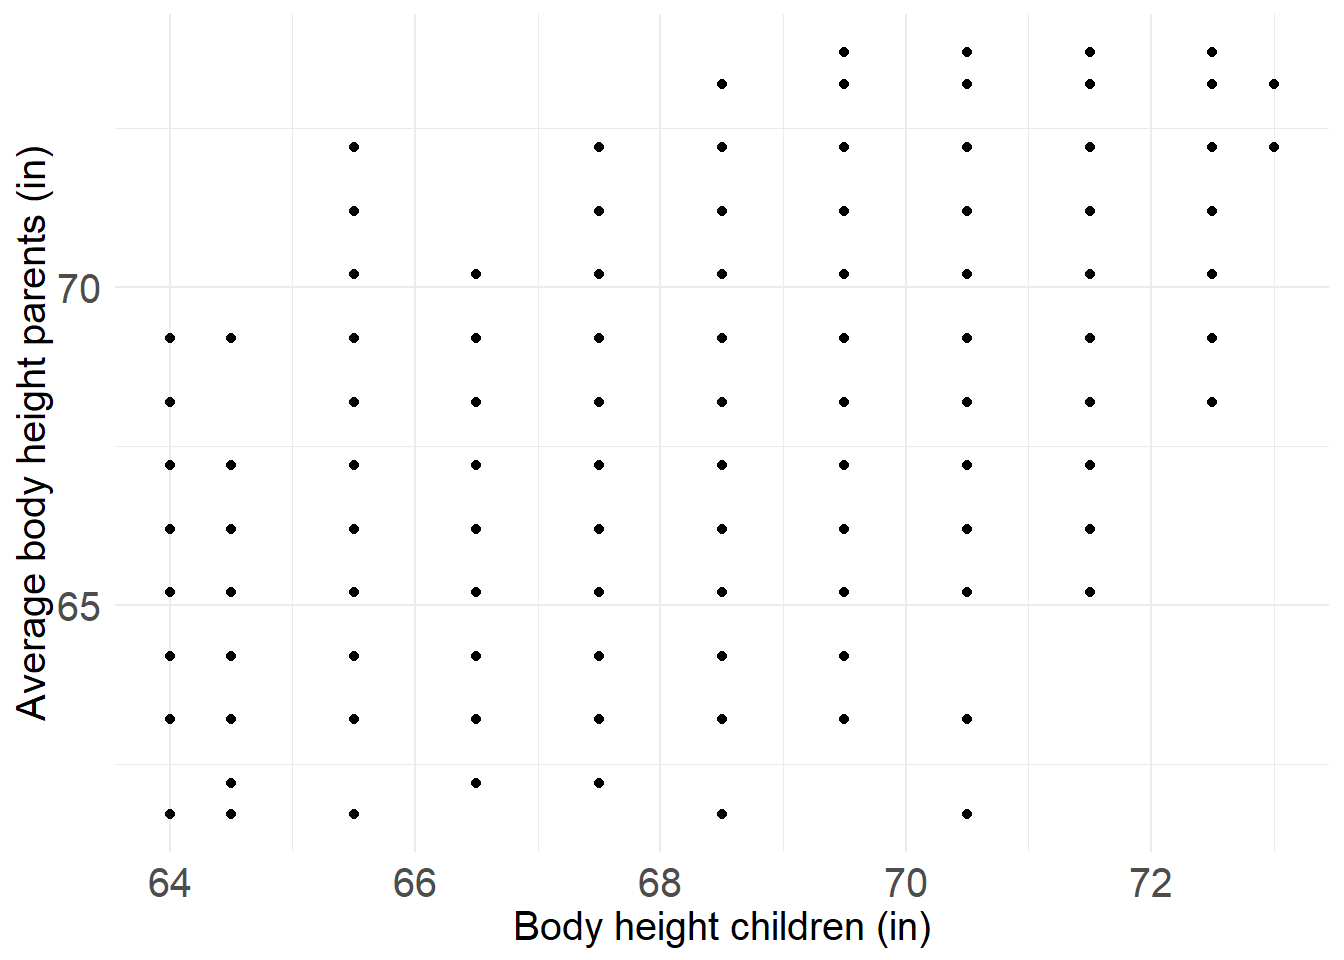
\includegraphics[width=0.5\linewidth]{outlier-detection_files/figure-latex/galton-1-1} \caption{Galton's heredity data in the \texttt{psych} package
\citep[dataset \texttt{galton}]{R-psych}}\label{fig:galton-1}
\end{figure}




Whereas taller parents had taller children, the offspring of
particularly tall parents was smaller than them wheareas smaller
parents' children had a relatively large body height. In an attempt to
characterize the connection he drew a line with a slope of 2/3.
\citep[p.~96f.]{Galton1889} Regression analysis has come a far way since
then. His successors determined the more rigorous method of least
squares to compute linear models. The slope determined by this method is
0.65; Galton's visual estimation\footnote{reproduced from Galton
  \citeyearpar[p.~96]{Galton1889}} had therefore been quite accurate.

\begin{figure}
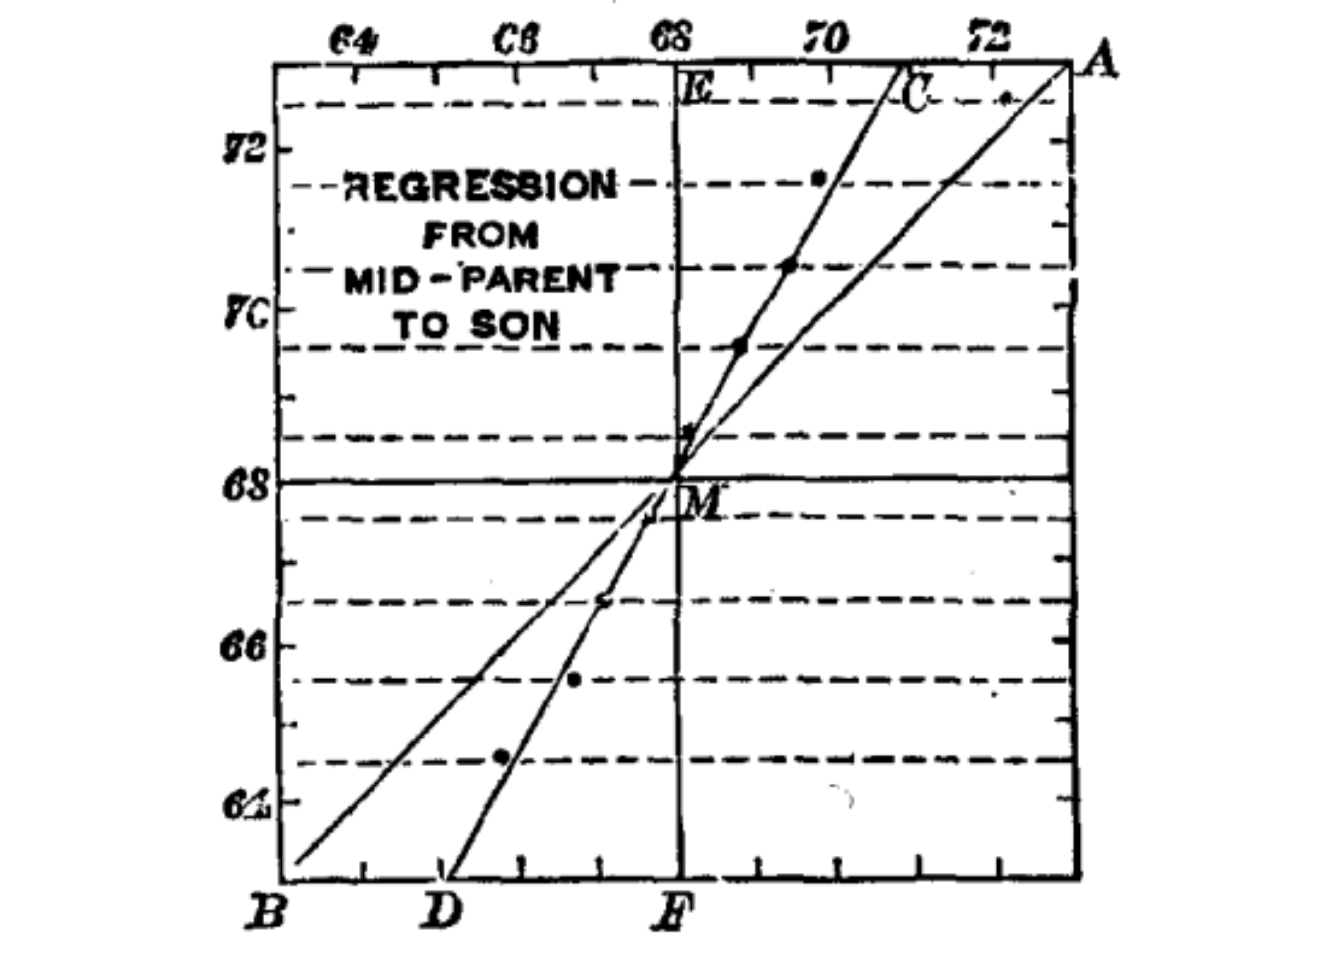
\includegraphics[width=0.5\linewidth]{outlier-detection_files/figure-latex/galton-2-1} 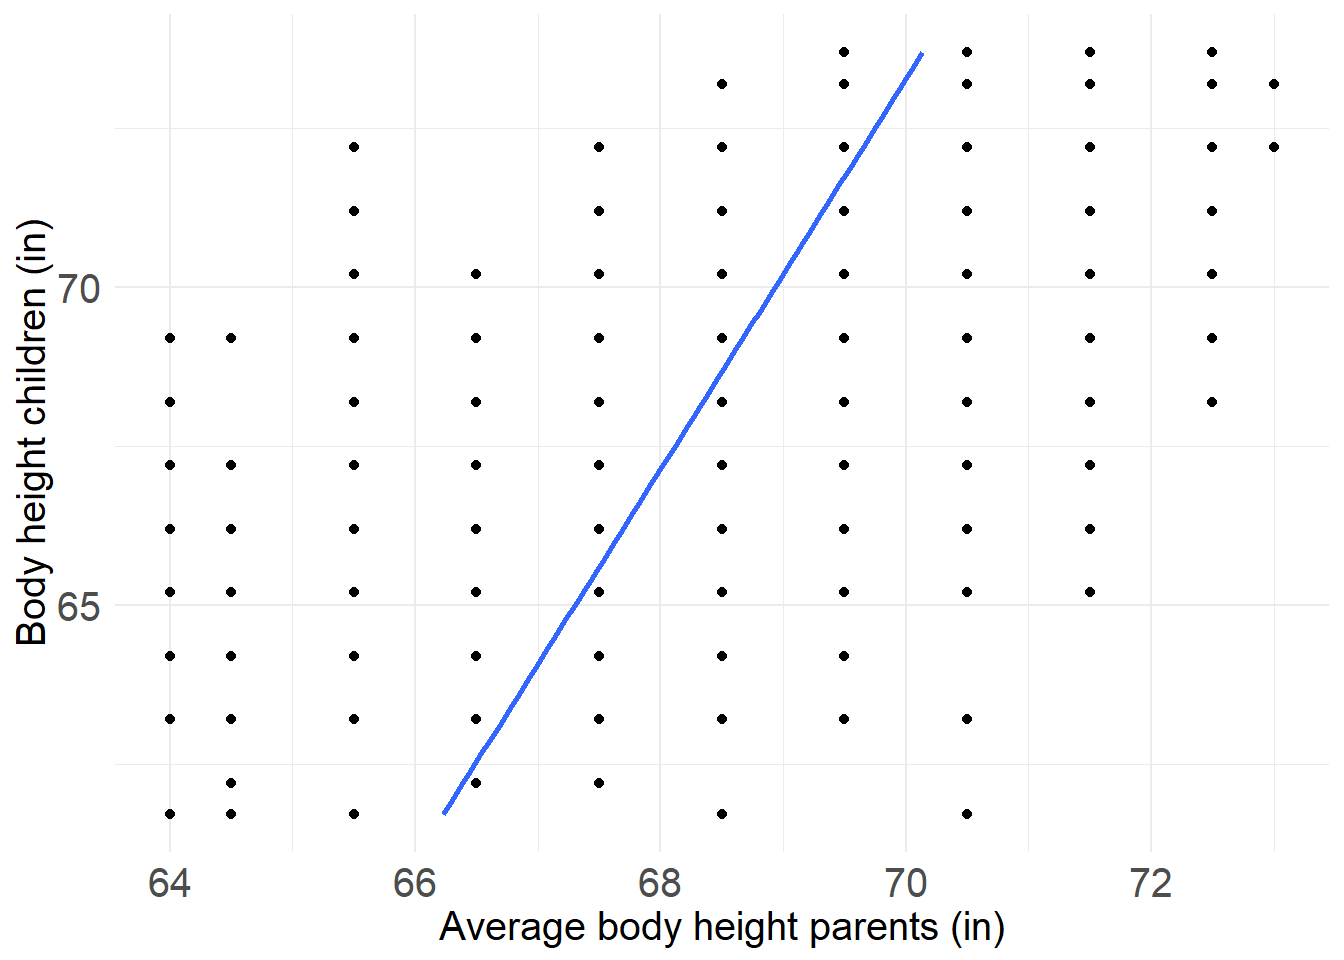
\includegraphics[width=0.5\linewidth]{outlier-detection_files/figure-latex/galton-2-2} \caption{Left: Galton's original estimation (the line connecting C
and D). Right: Least Squares linear model. Note that the x-axis now
represents the parents' height wheareas the childrens' height is drawn
on the y-axis.}\label{fig:galton-2}
\end{figure}






\chapter{Literature}\label{literature}

Here is a review of existing methods.

\chapter{Methods}\label{methods}

We describe our methods in this chapter.

\chapter{Applications}\label{applications}

Some \emph{significant} applications are demonstrated in this chapter.

\section{Example one}\label{example-one}

\section{Example two}\label{example-two}

\chapter{Final Words}\label{final-words}

We have finished a nice book.

\bibliography{outlier-detection.bib}


\end{document}
